\documentclass[border=4pt]{standalone}
\usepackage{tikz}
\usetikzlibrary{arrows.meta,positioning,topaths}
\tikzset{
  object/.style={draw,circle,minimum size=9mm,inner sep=1pt},
  upper morphism/.style={to path={(\tikztostart)
    .. controls +(12mm,9mm) and +(-12mm,9mm) .. (\tikztotarget) \tikztonodes}},
  lower morphism/.style={to path={(\tikztostart)
    .. controls +(12mm,-9mm) and +(-12mm,-9mm) .. (\tikztotarget) \tikztonodes}}
}
\begin{document}
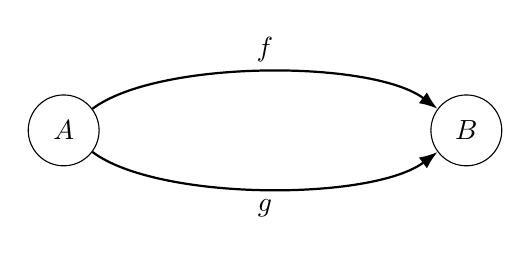
\begin{tikzpicture}[>=Latex,node distance=42mm]
  \node[object] (a) {$A$};
  \node[object,right=of a] (b) {$B$};
  \draw[->,thick,upper morphism] (a) to node[above] {$f$} (b);
  \draw[->,thick,lower morphism] (a) to node[below] {$g$} (b);
\end{tikzpicture}
\end{document}
